\documentclass[11pt, margin=17pt]{standalone} 
\usepackage{amsmath, amssymb}
\usepackage{ifthen}

\usepackage{tikz}
\usetikzlibrary{math, calc, arrows.meta}
\usetikzlibrary{decorations.markings}


\pgfkeys{/tikz/.cd,
  x bound start/.store in=\xBoundStart,
  x bound end/.store in=\xBoundEnd,
  y bound start/.store in=\yBoundStart,
  y bound end/.store in=\yBoundEnd
}

\makeatletter
\tikzset{%
  bounds/.style n args={4}{%
    evaluate={%
      \xBoundStart = #1;
      \xBoundEnd = #2;
      \yBoundStart = #3;
      \yBoundEnd = #4;
    }
  },
  pics/vector field background/.style={% axes + grid for a vector field
    code={%
      \begin{scope}[every node/.style={scale=.8},
        evaluate={%
          \iIni = {int(\xBoundStart)};
          \iEnd = {int(\xBoundEnd)};
          \jIni = {int(\yBoundStart)};
          \jEnd = {int(\yBoundEnd)};
        }]
        \draw[gray!50] (\xBoundStart, \yBoundStart)
        grid (\xBoundEnd, \yBoundEnd);
        \fill[black] (0, 0) circle (1pt);
        \foreach \i in {\iIni, ..., \iEnd}{%
          \path (\i, \yBoundStart) node[below=1ex] {$\i$};
        }
        \foreach \j in {\jIni, ..., \jEnd}{%
          \path (\xBoundStart, \j) node[left=1ex] {$\j$};
        }           
      \end{scope}
    }
  },
  flow/.style={%  create a directional arrow along a trajectory
    decoration={
      markings,% switch on markings
      mark=at position .5 with {\arrow[#1]{Latex}}
    }, postaction=decorate
  },
  -flow/.style={%
    decoration={
      markings,% switch on markings
      mark=at position .5 with {\arrowreversed[#1]{Latex}}
    }, postaction=decorate
  },
  runge-kutta/.style={%  to be invoked before using ode-trajectory, ...
    evaluate={%
      int \N@ode, \i, \j;
      \N@ode = 4;
      for \i in {1, ..., \N@ode}{%
        for \j in {1, ..., \N@ode}{%
          \a@ode{\i,\j} = 0;
        };
      };
      \a@ode{2,1} = 1/2; \a@ode{3,2} = 1/2; \a@ode{4,3} = 1;
      \c@ode{1} = 0; \c@ode{2} = 1/2; \c@ode{3} = 1/2; \c@ode{4} = 1;
      \b@ode{1} = 1/6; \b@ode{2} = 1/3; \b@ode{3} = 1/3; \b@ode{4} = 1/6;
    }
  },
  % for ode in two dimensions
  ode-trajectory/.style args={RHTx=#1, RHTy=#2, from=#3, to=#4, steps=#5}{%
    insert path={coordinate (tmp) let \p1 = (tmp) in},
    evaluate={%
      real \showpointr, \testTmp;
      \showpointr = 1;
      int \steps@ode, \i, \j, \k, \s;
      \t@ode{0} = #3;
      \u@ode{0} = \x1*0.0352778;  % converts pt to cm
      \v@ode{0} = \y1*0.0352778;
      \steps@ode = int(#5);
      \t@ode{\steps@ode} = #4;
      \h = (\t@ode{\steps@ode} -\t@ode{0})/\steps@ode;
      for \s in {1, 2, ..., \steps@ode}{
        \k = int(\s -1);
        \t@ode{0,1} = \t@ode{\k};
        \x@ode{0,1} = \u@ode{\k};
        \y@ode{0,1} = \v@ode{\k};
        \qx@ode{0,1} = #1(\t@ode{0,1}, \x@ode{0,1}, \y@ode{0,1});
        \qy@ode{0,1} = #2(\t@ode{0,1}, \x@ode{0,1}, \y@ode{0,1});
        for \i in {2, ..., \N@ode}{%
          \t@ode{0,\i} = \t@ode{\k} +\h*\c@ode{\i};
          \x@ode{0,\i} = \u@ode{\k};
          \y@ode{0,\i} = \v@ode{\k};
          for \j in {1, ..., {int(\i -1)}}{%
            \x@ode{0,\i} = \x@ode{0,\i} +\h*\a@ode{\i,\j}*\qx@ode{0,\j};
            \y@ode{0,\i} = \y@ode{0,\i} +\h*\a@ode{\i,\j}*\qy@ode{0,\j};
          };
          \qx@ode{0,\i} = #1(\t@ode{0,\i}, \x@ode{0,\i}, \y@ode{0,\i});
          \qy@ode{0,\i} = #2(\t@ode{0,\i}, \x@ode{0,\i}, \y@ode{0,\i});
        };
        \t@ode{\s} = \t@ode{\k} +\h;
        \u@ode{\s} = \u@ode{\k};
        \v@ode{\s} = \v@ode{\k};
        for \i in {1, 2, ..., \N@ode}{%
          \u@ode{\s} = \u@ode{\s} +\h*\b@ode{\i}*\qx@ode{0,\i};
          \v@ode{\s} = \v@ode{\s} +\h*\b@ode{\i}*\qy@ode{0,\i};
        };
      };
      \k = \steps@ode-1;
      \testTmp = pow(pow(\u@ode{\steps@ode} -\u@ode{\k}, 2)
      +pow(\v@ode{\steps@ode} -\v@ode{\k}, 2), .5);
    },
    insert path={%
      \foreach \s in {1, ..., \steps@ode}{
        -- (\u@ode{\s}, \v@ode{\s})
      }
    }
  },
  m vector field/.style n args={5}{% u / v / Nx / Ny / arrow scale
    insert path = {%
      \pgfextra{%
        \let\tikz@mode@save=\tikz@mode
        \let\tikz@options@save=\tikz@options%
      }
    },
    evaluate={%
      coordinate \tmp@P, \tmp@V;
      integer \Nx, \Ny;
      \Nx = #3;
      \Ny = #4;
      real \dx, \dy, \tmp, \uVF, \vVF, \nVF, \s@cst;
      \s@cst = .49;
      \dx = (\xBoundEnd -\xBoundStart)/\Nx;
      \dy = (\yBoundEnd -\yBoundStart)/\Ny;
      for \i in {1, ..., \Nx}{%
        for \j in {1, ..., \Ny}{%
          \uVF = #1(\xBoundStart -\dx/2 +\i*\dx, \yBoundStart -\dy/2 +\j*\dy);
          \vVF = #2(\xBoundStart -\dx/2 +\i*\dx, \yBoundStart -\dy/2 +\j*\dy);
          \nVF = pow(\uVF*\uVF +\vVF*\vVF, .5);
          if  \nVF > \s@cst then {%
            \uVF = \uVF/\nVF*.5;
            \vVF = \vVF/\nVF*.5;
          };
          \tmp@P = (\xBoundStart +\i*\dx, \yBoundStart +\j*\dy);
          \tmp@V = (#5*\uVF, #5*\vVF);
          {
            \draw[arrows={-Latex[width=2.5pt, length=2pt]}]
            \pgfextra{\let\tikz@mode=\tikz@mode@save
              \let\tikz@options=\tikz@options@save}
            ($(\tmp@P) -.5*(\tmp@V)$) -- ++(\tmp@V);
          };          
        };
      };
    }
  }
}
\newcommand{\streamPlot}[7]{% RHTx, RHTy, h, px, py, min, color
  \tikzmath{%
    integer \steps@ode, \i, \j, \k, \s\, flag;
    real \h, \nor;
    \flag = 0;
    \s = 0;
    \k = 0;
    \h = #3;    
    \u@ode{0} = #4;
    \v@ode{0} = #5;
    \t@ode{0} = 0;
  },
  \whiledo{\equal{\flag}{0}}{%
    \tikzmath{
      \s = \s +1;
      \t@ode{0,1} = 0;
      \x@ode{0,1} = \u@ode{\k};
      \y@ode{0,1} = \v@ode{\k};
      \qx@ode{0,1} = #1(\t@ode{0,1}, \x@ode{0,1}, \y@ode{0,1});
      \qy@ode{0,1} = #2(\t@ode{0,1}, \x@ode{0,1}, \y@ode{0,1});
      for \i in {2, ..., \N@ode}{%
        \t@ode{0,\i} = \t@ode{\k} +\h*\c@ode{\i};
        \x@ode{0,\i} = \u@ode{\k};
        \y@ode{0,\i} = \v@ode{\k};
        for \j in {1, ..., {int(\i -1)}}{%
          \x@ode{0,\i} = \x@ode{0,\i} +\h*\a@ode{\i,\j}*\qx@ode{0,\j};
          \y@ode{0,\i} = \y@ode{0,\i} +\h*\a@ode{\i,\j}*\qy@ode{0,\j};
        };
        \qx@ode{0,\i} = #1(\t@ode{0,\i}, \x@ode{0,\i}, \y@ode{0,\i});
        \qy@ode{0,\i} = #2(\t@ode{0,\i}, \x@ode{0,\i}, \y@ode{0,\i});
      };
      \t@ode{\s} = \t@ode{\k} +\h;
      \u@ode{\s} = \u@ode{\k};
      \v@ode{\s} = \v@ode{\k};
      for \i in {1, 2, ..., \N@ode}{%
        \u@ode{\s} = \u@ode{\s} +\h*\b@ode{\i}*\qx@ode{0,\i};
        \v@ode{\s} = \v@ode{\s} +\h*\b@ode{\i}*\qy@ode{0,\i};
      };
      \nor = pow(%
        pow(\u@ode{\s} -\u@ode{\k}, 2) +pow(\v@ode{\s} -\v@ode{\k}, 2),
      .5);
      if \nor<#6 then {\flag = 1;};
      if \u@ode{\s}<\xBoundStart then {\flag = 1;};
      if \u@ode{\s}>\xBoundEnd then {\flag = 1;};
      if \v@ode{\s}<\yBoundStart then {\flag = 1;};
      if \v@ode{\s}>\yBoundEnd then {\flag = 1;};
      \k = \k +1;
    }
  },
  \tikzmath{%
    if \s>1 then {%
      if #3>0 then {%
        {%
          \draw[#7, flow={#7}]  (\u@ode{0}, \v@ode{0})
          \foreach \i [parse=true] in {1, ..., \s-1}{
            -- (\u@ode{\i}, \v@ode{\i})
          };
        };
      } else {%
        {%
          \draw[#7, -flow={#7}]  (\u@ode{0}, \v@ode{0})
          \foreach \i [parse=true] in {1, ..., \s-1}{
            -- (\u@ode{\i}, \v@ode{\i})
          };
        };
      };
    };
  }
}
\makeatother

\tikzset{
  pics/stream plot by name/.style args={RHTx=#1, RHTy=#2, dT=#3, pName=#4,
    pNumber=#5, min=#6, color=#7}{%
    code={
      \foreach \i in {1, ..., #5}{%
        \tikzmath{%
          coordinate \P;
          \P = (#4-\i);
          \px = \Px*1pt/1cm;  % converts pt to cm
          \py = \Py*1pt/1cm;
        }
        % \draw (\px, \py) circle (2pt);
        \streamPlot{#1}{#2}{#3}{\px}{\py}{#6}{#7};
        \streamPlot{#1}{#2}{-#3}{\px}{\py}{#6}{#7};
      }
    }
  },
  pics/stream plot TB/.style args={%
    RHTx=#1, RHTy=#2, dT=#3, uSteps=#4, min=#5, color=#6}{%
    code={
      \tikzmath{%
        real \px, \py, \dx;
        \dx = (\xBoundEnd -\xBoundStart)/#4;
      }
      \foreach \i in {0, ..., #4}{%
        \tikzmath{%
          \px = \xBoundStart +\i*\dx;
          \py = \yBoundStart;
        }
        \streamPlot{#1}{#2}{#3}{\px}{\py}{#5}{#6};
        \streamPlot{#1}{#2}{-#3}{\px}{\py}{#5}{#6};
      }
      \foreach \i in {0, ..., #4}{%
        \tikzmath{%
          \px = \xBoundStart +\i*\dx;
          \py = \yBoundEnd;
        }
        \streamPlot{#1}{#2}{#3}{\px}{\py}{#5}{#6};
        \streamPlot{#1}{#2}{-#3}{\px}{\py}{#5}{#6};
      }
    }
  }
}


\begin{document}

%\iffalse
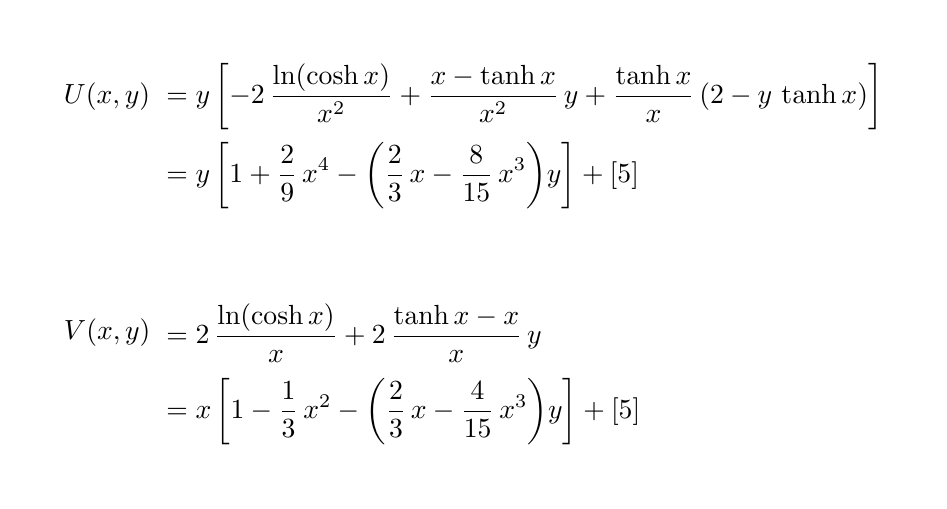
\begin{tikzpicture}[every node/.style={%
    right, align=left, inner sep=3ex
  }]
  \path (-1.3, 0) node {$U(x, y)$}
  (0, 0) node[] {$\displaystyle
    = y\left[
      -2\,\frac{\ln(\cosh x)}{x^2}
      +\frac{x -\tanh x}{x^2}\,y
      +\frac{\tanh x}{x}\,(2 -y\,\tanh x)
    \right]$}
  ++(0, -1) node[] {$\displaystyle
    = y\left[
      1 +\frac{2}{9}\,x^4
      -\bigg(\frac{2}{3}\,x -\frac{8}{15}\,x^3\bigg)y
    \right] +[5]$};

  \path (-1.3, -3) node {$V(x, y)$}
  (0, -3) node[] {$\displaystyle
    = 2\,\frac{\ln(\cosh x)}{x} +2\,\frac{\tanh x -x}{x}\,y$}
  ++(0, -1) node[] {$\displaystyle
    = x\left[
      1 -\frac{1}{3}\,x^2
      -\bigg( \frac{2}{3}\,x -\frac{4}{15}\,x^3 \bigg)y
    \right] +[5]$};
\end{tikzpicture}
%\fi


\tikzmath{%
  function Ux(\t, \u, \v) {%
    real \a, \b, \c;
    if abs(\u)>.05 then {%
      \a = -2*ln(cosh(\u))/(\u*\u);
      \b = (\u -tanh(\u))/(\u*\u)*\v;
      \c = (tanh(\u)/\u)*(2 - tanh(\u)*\v);
    } else {%
      \a = 1 -2/3*\u*\v;
      \b = 8/15*pow(\u, 3)*\v;
      \c = 2/9*pow(\u, 4);
    };
    return {(\a +\b +\c)*\v};
  };
  function Uy(\t, \u, \v) {%
    real \a, \b;
    if abs(\u)>.05 then {%
      \a = ln(cosh(\u))/\u;
      \b = (tanh(\u) -\u)/\u;
      return {2*\a +2*\b*\v};
    } else {
      \a = 1 -pow(\u, 2)/3;
      \b = -(2/3)*\u +(4/15)*pow(\u, 3);
      return {\u*(\a +\b*\v)};
    };
  };
  function fUy(\u) {%
    real \a, \b;
    \a = ln(cosh(\u))/\u;
    \b = (\u -tanh(\u))/\u;
    return \a/\b;
  };
  function UxVF(\u, \v) {%
    real \a, \b, \c;
    if abs(\u)>.05 then {%
      \a = -2*ln(cosh(\u))/(\u*\u);
      \b = (\u -tanh(\u))/(\u*\u)*\v;
      \c = (tanh(\u)/\u)*(2 - tanh(\u)*\v);
    } else {%
      \a = 1 -2/3*\u*\v;
      \b = 8/15*pow(\u, 3)*\v;
      \c = 2/9*pow(\u, 4);
    };
    return {(\a +\b +\c)*\v};
  };
  function fUx(\u) {%
    real \a, \b;
    \a = 2*(tanh(\u)/\u) -2*ln(cosh(\u))/(\u*\u);
    \b = -(\u -tanh(\u))/(\u*\u) +(tanh(\u)/\u)*tanh(\u);
    return \a/\b;
  };
  function UyVF(\u, \v) {%
    real \a, \b;
    if abs(\u)>.05 then {%
      \a = ln(cosh(\u))/\u;
      \b = (tanh(\u) -\u)/\u;
      return {2*\a +2*\b*\v};
    } else {
      \a = 1 -pow(\u, 2)/3;
      \b = -(2/3)*\u +(4/15)*pow(\u, 3);
      return {\u*(\a +\b*\v)};
    };
  };
}

\iffalse
\begin{tikzpicture}
  \draw[gray!50, very thin] (-3.5, -3.25) grid (3.5, 3.25);
  \draw[->] (-3.5, 0) -- (3.5, 0) node[above right] {$x$};
  \draw[->] (0,-3.5) -- (0, 3.5) node[left] {$y$};
  
  \draw[blue!70!black, thick, variable=\t, domain=.5:3.25, samples=200]
  plot (\t, {fUx(\t)});
  \draw[blue!70!black, thick] (-3.25, 0) -- (3.25, 0);
  \draw[blue!70!black, thick, variable=\t, domain=-3.25:-.5, samples=200]
  plot (\t, {fUx(\t)});
  \draw[red, thin, variable=\t, domain=.5:3.25, samples=200]
  plot (\t, {fUy(\t)});
  \draw[red] (-0, -3.25) -- (0, 3.25);
  \draw[red, thin, variable=\t, domain=-3.25:-.5, samples=200]
  plot (\t, {fUy(\t)});
\end{tikzpicture}
\fi

\iffalse
\begin{tikzpicture}[runge-kutta, bounds={-4}{4}{-4}{4}, scale=1.2]
  \path pic[scale=1.2] {vector field background};

  \draw[blue!70!black, thick,
  variable=\t, domain=.35:\xBoundEnd, samples=200]
  plot (\t, {fUx(\t)});
  \draw[blue!70!black, thick] (\xBoundStart, 0) -- (\xBoundEnd, 0);
  \draw[blue!70!black, thick,
  variable=\t, domain=\xBoundStart:-.35, samples=200]
  plot (\t, {fUx(\t)});
  \draw[red, thin, variable=\t, domain=.35:\xBoundEnd, samples=200]
  plot (\t, {fUy(\t)});
  \draw[red] (-0, \xBoundStart) -- (0, \xBoundEnd);
  \draw[red, thin, variable=\t, domain=\xBoundStart:-.35, samples=200]
  plot (\t, {fUy(\t)});
  \draw[green!50!black, thick, m vector field={UxVF}{UyVF}{35}{35}{.4}];
\end{tikzpicture}
\fi

\iffalse
\begin{tikzpicture}[runge-kutta, bounds={-4}{4}{-3.5}{3.5}]
  \path pic {vector field background};

  % A points
  \path (0, 1.5) coordinate (A-1);
  \path (0, -1.5) coordinate (A-2);
  \path (2.2, \yBoundEnd) coordinate (A-3);
  \path (-2.2, \yBoundStart) coordinate (A-4);

  % B points
  \tikzmath{
    integer \N;
    \N = 4;
  }
  \foreach \i in {1, ..., \N}{%
    \path (\i*360/\N: .5) coordinate (B-\i);
  }

  \path pic {stream plot by name={RHTx=Ux, RHTy=Uy, dT=.05,
      pName=A, pNumber=4, min=.005, color=blue!60!black}};
  \path pic {stream plot by name={RHTx=Ux, RHTy=Uy, dT=.05,
      pName=B, pNumber=\N, min=.005, color=blue!60!black}};

  \path pic {stream plot TB={RHTx=Ux, RHTy=Uy, dT=.05,
      uSteps=11, min=.005, color=blue!60!black}};

  \draw[red, very thick] (2.7, -3)
  [ode-trajectory={RHTx=Ux, RHTy=Uy, from=0, to=15, steps=1500}];  
\end{tikzpicture}
\fi

\end{document}